\section{Background}
\label{sec:background}

There are three main factors that determine the operational performance of an autonomous mobility on demand (AMoD) system.

\begin{enumerate}
\item The fleet size $N$ has large influence on wait times and vehicle availbility. Large fleet sizes effectively decrease the passenger wait times but also cause higher capital expeditures for the operator.
\item The dispatching strategy, i.e. the assignment of available vehicles to waiting passengers heavily influences the performance. Figures \ref{fig:dispatch-subopt} and \ref{fig:dispatch-opt} show suboptimal and optimal rebalancing choices.
\item The rebalancing strategy, i.e. the repositioning of available vehicles when there is no customer present. If vehicles are rebalanced often, it may increase the service level of the system, but it may also increase the total empty distance driven by the vehicles and thus the operational cost for the operator, see figure \ref{fig:dispatch-optreb} for an illustration.
\end{enumerate}



\begin{figure}[h]
    \centering
    \begin{subfigure}[b]{0.3\textwidth}
        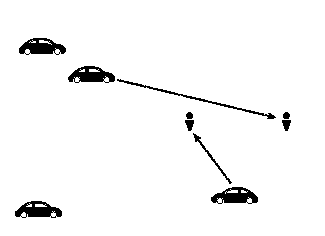
\includegraphics[width=\textwidth]{figures/RebalancingRedispatching1}
        \caption{Dispatching command with non-minimal summed pickup distance.}
        \label{fig:dispatch-subopt}
    \end{subfigure}
    ~ %add desired spacing between images, e. g. ~, \quad, \qquad, \hfill etc.
      %(or a blank line to force the subfigure onto a new line)
    \begin{subfigure}[b]{0.3\textwidth}
        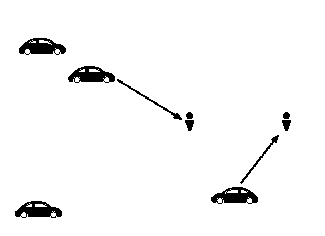
\includegraphics[width=\textwidth]{figures/RebalancingRedispatching2}
        \caption{Dispatching command with minimal summed pickup distance.}
        \label{fig:dispatch-opt}
    \end{subfigure}
    ~ %add desired spacing between images, e. g. ~, \quad, \qquad, \hfill etc.
    %(or a blank line to force the subfigure onto a new line)
    \begin{subfigure}[b]{0.3\textwidth}
        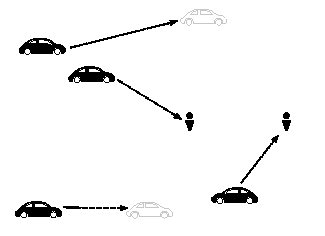
\includegraphics[width=\textwidth]{figures/RebalancingRedispatching3}
        \caption{Dispatching command with minimal summed pickup distance and rebalancing.}
        \label{fig:dispatch-optreb}
    \end{subfigure}
    \caption{Dispatching and Rebalancing Strategies}\label{fig:animals}
\end{figure}


Furthermore there is a charging and service process for the vehicles that influences the operational performance as well as parameters not related to the operation of vehicles (e.g. cleaning, interior design,...).

As there is a complex interaction between the fleet size, the amount of rebalancing, the operational strategies (dispatching and rebalancing), the service level and the costs for the operator, in \ref{subsec:performancemeasures} we propose what variables and charts to analyze to analyze the performance for AMoD systems.



\subsection{Performance of Autonomous Mobility on Demand Systems}
\label{subsec:performancemeasures}

The service level is mainly dependant on the customer wait times. We define the wait time as the time from the arrival of a taxi request to the system until an available vehicle has reached the spot. For a given fleet size, the distribution of wait times is analyzed for every time step of the day (see XYZ include figure). Furthermore the waiting time has to be analyzed as a function of the fleet size $N$, see e.g. XYZ include figure.

The operational cost that can be influenced with the choice of the operating strategy is mainly based on the driven distance. We distinguish three types of distances. Vehicles can either drive to pickup a customer, they can drive to rebalance or they can drive with a customer. Assuming a pricing scheme where customers pay for distance driven and time spent in the vehicle, the distance driven with customers can be assumed to be profitable distance. Furthermore the total distance driven with customers is contant when considering a fixed set of customer requests and assuming that vehicles travel the minimum distance path for each request in the network.

Thus the goal of each operational strategy is to minimize the total empty distance (pickup and rebalancing) by the vehicles. As shown in \cite{treleaven2011asymptotically} this distance cannot be driven to zero for general demand patterns, it is bounded below by the earth mover's distance which is a measure of how different the distribution of origins and destinations are in each time step, see e.g. \cite{ruschendorf1985wasserstein}. The earth mover's distance for the Zurich scenario considered in this work calculated for hourly time bins is shown in figure \ref{fig:EMD}.


\begin{figure}[h]
\begin{center}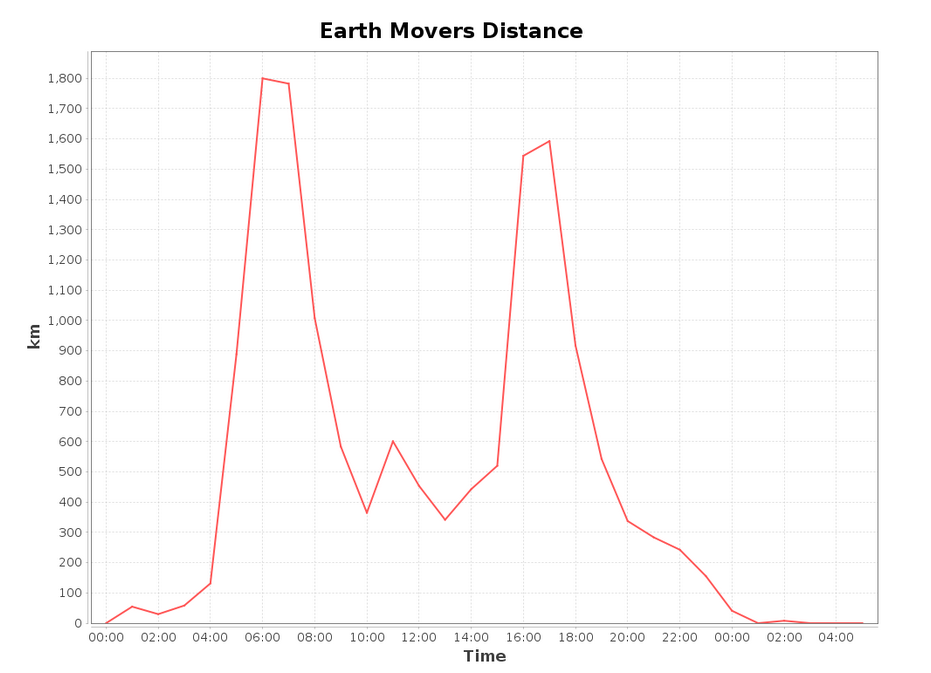
\includegraphics[width=0.9\textwidth]{figures/EMDZurich.png}\end{center}
\caption{Earth mover's distance for Zurich calculated for hourly time bins. XYZ make figure nicer.}
\label{fig:EMD}
\end{figure}

While the total amount of empty distance driven can not be reduced to zero, the ratio of pickup and rebalance distance driven can be influenced by the controller. A well-performing fleet controller will reposition vehicles already before the demand appears, i.e. it will increase the rebalance distance but reduce the pickup distance. Perfect estimation of future demands would lead to a system where almost all of the empty distance is rebalance distance. In order to make these concepts visible, we propose the plot in figure \ref{fig:study_area_vnodes} to assess the operational quality of an AMoD system. Distances that are profitable and cannot be avoided are plotted on the negative ordinate and empty distances on the positive ordinate. Furthermore the empty distances are distinguished into rebalancing and pickup distances. Any controller tries to minimize the area above the abscissa, ensure it is composed mostly of rebalancing distances and satisfy certain service level constraints.



\begin{figure}[h]
\begin{center}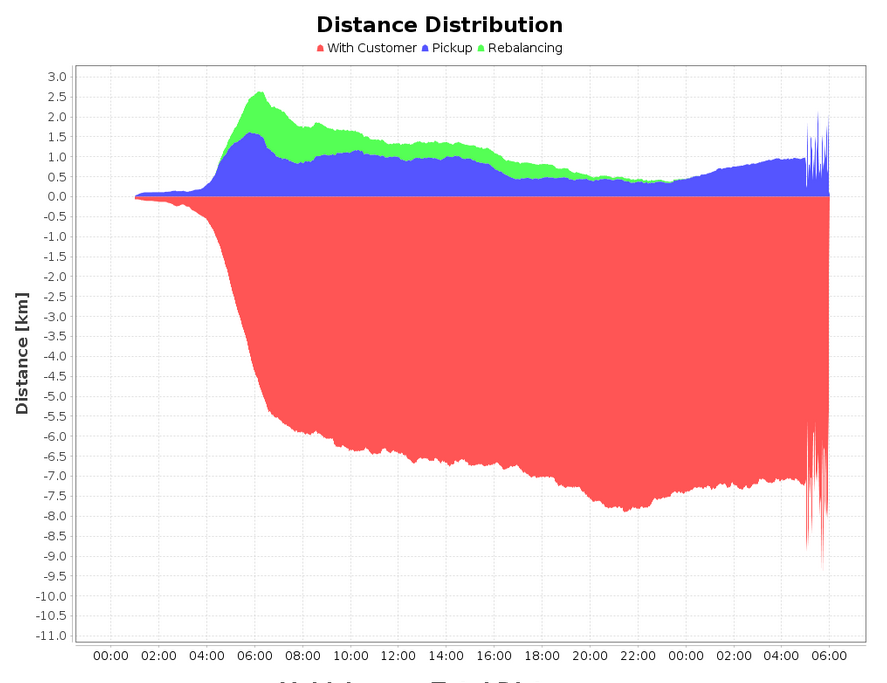
\includegraphics[width=0.9\textwidth]{figures/distancePlot.png}\end{center}
\caption{Distances with customer, pickup distances and rebalancing distances driven by the fleet in every time step. INCLUDE ANOTHER FIGURE or refence to actual figure shown in simulations XZY}
\label{fig:study_area_vnodes}
\end{figure}




\subsection{Automatic Control of Autonomous Mobility on Demand Systems}
\label{subsec:automaticControl}

In this work we analyze four different operating strategies from literature for the Zurich scenario, which are briefly outlined below:

\begin{enumerate}
\item The single heuristic dispatcher is the strategy presented in \cite{bischoff2016simulation}. In every dispatching time step $\delta t_D$ If there are more available vehicles than requests, it iterates on the list of requests and assigns to each request the closest vehicle. If there are more open requests than available vehicles, the controller iterates on the available vehicles and assigns the closest open request to each vehicle. The assignments are binding, i.e. they are not reopened once concluded.
\item The global Euclidean bipartite matching dispatcher determines an optimal bipartite matching between all open requests and available vehicles in every dispatching time step $\delta t_D$. The used distance function is the Euclidean distance which allows to use fast algorithms, e.g. \cite{agarwal2004near}. In contrast to the previous strategy, the assignments can be changed until a vehicle actually reaches its target. If arrival probabilties for future time steps is taken into account, this strategy can be considered as the optimal dispatching strategy based on Euclidean distances.
\item In \cite{pavone2011load} a feedforward strategy is presented on how to rebalance vehicles between different vertices in a directed graph $G = (V,E)$. For each vertex $i$ and time step $\delta_t$, the arrival rates $\lambda_i$ and transition probabilities $p_{ij}$ for any nodes $v_i, v_j \in V$  are used in a linear program to compute the optimal rebalancing flows $\alpha _{ij}$ in that time step assuming that the system is at equilibrium. To implement this strategy, we divided the city of Zurich into a set of areas. The nodes from \cite{pavone2011load} represent the centroids of these areas on which a complete directed graph called virtual network is placed, see figure \ref{fig:virtualNetwork}. Available cars are continuously rebalanced between the vertices of the virtual network according to the static rebalancing rates $\alpha_{ij}$. As the work does not detail the proposed dispatching algorithm for this strategy, we match cares using global Euclidean bipartite matching. Rebalancing vehicles cannot be dispatched until they reach their destination.
\item The last implemented strategy is as well derived from \cite{pavone2011load}. Instead of a pure feedforward solution, here in every rebalancing timestep $\delta t_R$ for every area of the virtual network the avaialble cars and open requests are counted and fed into an integer linear program which calculates the number of cars $reb _{ij}$ to be sent from virtual vertex $i$ to virtual vertex $j$. As in the feedforward strategy, the matching of the cars is done via global Euclidean bipartite matching.
\end{enumerate}



\begin{figure}[h]
\begin{center}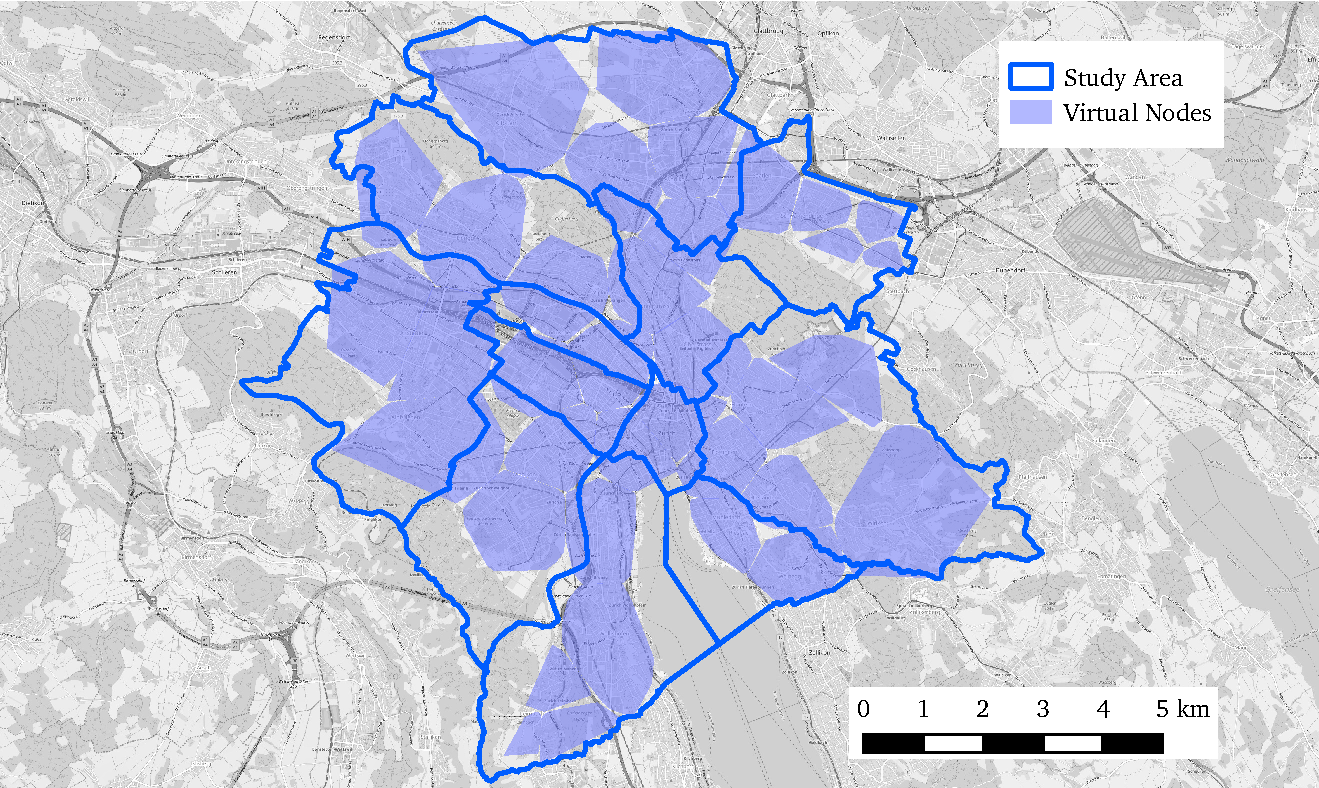
\includegraphics[width=1.0\textwidth]{figures/map.pdf}\end{center}
\caption{The study area covering the 12 districts of Zurich and the nodes of the virtual network for the rebalancing algorithms.}
\label{fig:study_area_vnodes}
\end{figure}

\subsection{Fleet sizing for Zurich}
\label{subsec:fleetSizing}

In this section we use strategies presented in \cite{spieser2014toward} to estimate the needed fleet size for a given scenario without actually using a simulation. We then compare these values to the simulation results in section XZY.

We define an AMoD system to be stable if the number of open requests is bounded for all times. A necessary condition for this to hold is that the distance the vehicles can drive collectively is larger than the distance to be driven to satisfy new requests entering the system. For every time step $k = 0,1,2,...,T$ over the course of a simulation we can define these quantities as $N \cdot v_k$ and $ \lambda_k \cdot d_{av,k}$ respectively, where $v_k$ is the average vehicle speed in time step $k$, $\lambda_k$ the customer arrival rate in timestep $k$ and $d_{av,k}$ the average distance per request in timestep $k$. Summing over the day, rearranging and using the fact that the average distance per trip is composed of the actual trip distance and the earth mover's distance, we can state that

\begin{align}
N \geq \frac{\lambda_k \cdot (d_{OD,k} + d_{EMD,k} )}{v_k}
\end{align}

where $d_{OD,k}$ and $d_{EMD,k}$ are the averge driving distance per request and the average earth mover's distance per request in timestep $k$ respectively. The analysis conducted on the scneario data yields a minimum fleet size of XZY for Zurich.

This number presents a lower bound for the fleet size such that the system can be stable, however it does not show what fleet sizes are necessary for an acceptable level of service. In order to estimate this number we used the strategy presented in \cite{spieser2014toward} where data of the requests is used to compute the vehicle availabilities using mean value analysis in a closed Jackson network for different fleet sizes. The availability of a node is defined as the probability that there is at least one vehicle waiting at the node. Computing this quantity for every node of a virtual network for Zurich  XZY include information on timestep XZY and taking the average of all stations, we can generate the following figure:




\begin{figure}[h]
\begin{center}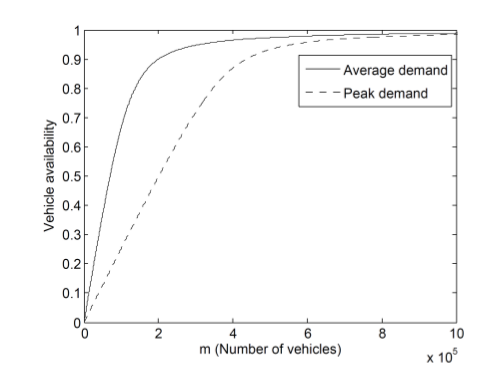
\includegraphics[width=0.9\textwidth]{figures/performancePlot.png}\end{center}
\caption{Performance driven fleet sizing for the city of Zurich according to \cite{spieser2014toward}. XZY put real plot}
\label{fig:performanceFleetSize}
\end{figure}

The results indicate that XZY include conclusion. XZY.
